\qns{Bode diagram of a transfer function.}
\qcontributor{Geoffrey N\'egiar}


\begin{enumerate}
\qitem \textbf{Plot the magnitude and phase of the following transfer function using the Bode approximation and a numerical solver and compare the two.}

\[ H(\omega) = \frac{100 \left(1 + j\frac{\omega}{1000}\right)}{\left(1 + j\frac{\omega}{10^6}\right)\left(1 + j\frac{\omega}{10^8}\right)} \]

We see 1 zero at $10^3 \si{\radian\per\second}$, 2 poles at $10^6 \si{\radian\per\second}$ and $10^8 \si{\radian\per\second}$, and a constant gain of 100. We start with the constant value, and then move from lowest to highest frequency plotting the poles and zeros as we go. Finally, we add together the plots for each of the individual poles and zeros to give us the final Bode plot.


\begin{figure}[H]
  \centering
  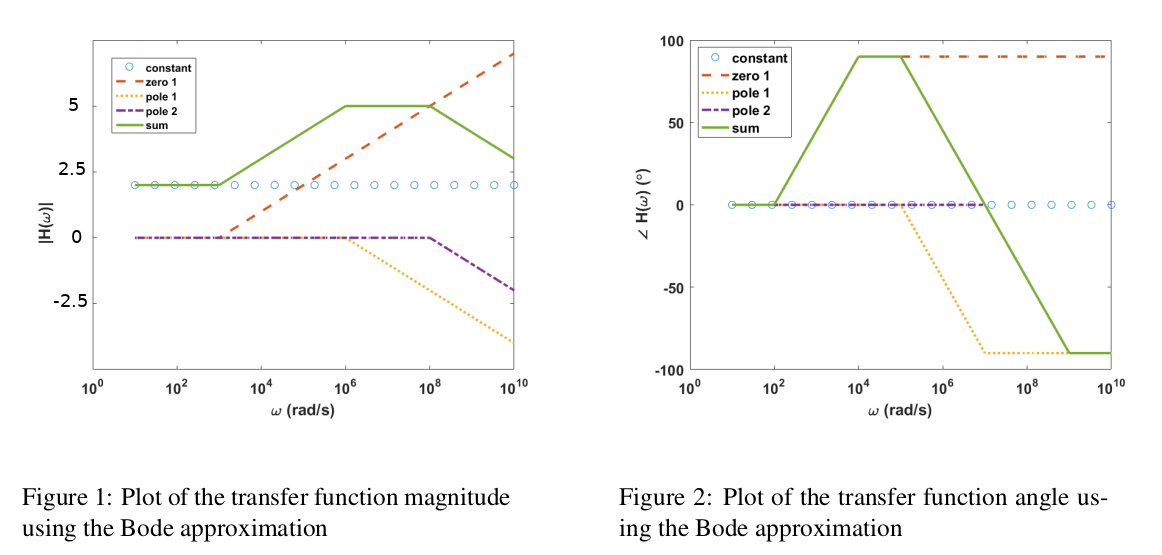
\includegraphics[scale=0.5]{figures/q_transfer_to_bode.png}
\end{figure}

Finally, comparing the Bode approximation and the precise value calculated via a computer, we can see the Bode approximation is very similar to the exact answer, except around the pole and zero frequencies (as expected).

\begin{figure}[H]
    \centering
    %% Creator: Matplotlib, PGF backend
%%
%% To include the figure in your LaTeX document, write
%%   \input{<filename>.pgf}
%%
%% Make sure the required packages are loaded in your preamble
%%   \usepackage{pgf}
%%
%% Figures using additional raster images can only be included by \input if
%% they are in the same directory as the main LaTeX file. For loading figures
%% from other directories you can use the `import` package
%%   \usepackage{import}
%% and then include the figures with
%%   \import{<path to file>}{<filename>.pgf}
%%
%% Matplotlib used the following preamble
%%   \usepackage[utf8x]{inputenc}
%%   \usepackage[T1]{fontenc}
%%
\begingroup%
\makeatletter%
\begin{pgfpicture}%
\pgfpathrectangle{\pgfpointorigin}{\pgfqpoint{4.550000in}{2.812055in}}%
\pgfusepath{use as bounding box, clip}%
\begin{pgfscope}%
\pgfsetbuttcap%
\pgfsetmiterjoin%
\definecolor{currentfill}{rgb}{1.000000,1.000000,1.000000}%
\pgfsetfillcolor{currentfill}%
\pgfsetlinewidth{0.000000pt}%
\definecolor{currentstroke}{rgb}{1.000000,1.000000,1.000000}%
\pgfsetstrokecolor{currentstroke}%
\pgfsetdash{}{0pt}%
\pgfpathmoveto{\pgfqpoint{0.000000in}{0.000000in}}%
\pgfpathlineto{\pgfqpoint{4.550000in}{0.000000in}}%
\pgfpathlineto{\pgfqpoint{4.550000in}{2.812055in}}%
\pgfpathlineto{\pgfqpoint{0.000000in}{2.812055in}}%
\pgfpathclose%
\pgfusepath{fill}%
\end{pgfscope}%
\begin{pgfscope}%
\pgfsetbuttcap%
\pgfsetmiterjoin%
\definecolor{currentfill}{rgb}{1.000000,1.000000,1.000000}%
\pgfsetfillcolor{currentfill}%
\pgfsetlinewidth{0.000000pt}%
\definecolor{currentstroke}{rgb}{0.000000,0.000000,0.000000}%
\pgfsetstrokecolor{currentstroke}%
\pgfsetstrokeopacity{0.000000}%
\pgfsetdash{}{0pt}%
\pgfpathmoveto{\pgfqpoint{0.710575in}{1.698391in}}%
\pgfpathlineto{\pgfqpoint{4.365000in}{1.698391in}}%
\pgfpathlineto{\pgfqpoint{4.365000in}{2.627055in}}%
\pgfpathlineto{\pgfqpoint{0.710575in}{2.627055in}}%
\pgfpathclose%
\pgfusepath{fill}%
\end{pgfscope}%
\begin{pgfscope}%
\pgfsetbuttcap%
\pgfsetroundjoin%
\definecolor{currentfill}{rgb}{0.000000,0.000000,0.000000}%
\pgfsetfillcolor{currentfill}%
\pgfsetlinewidth{0.803000pt}%
\definecolor{currentstroke}{rgb}{0.000000,0.000000,0.000000}%
\pgfsetstrokecolor{currentstroke}%
\pgfsetdash{}{0pt}%
\pgfsys@defobject{currentmarker}{\pgfqpoint{0.000000in}{-0.048611in}}{\pgfqpoint{0.000000in}{0.000000in}}{%
\pgfpathmoveto{\pgfqpoint{0.000000in}{0.000000in}}%
\pgfpathlineto{\pgfqpoint{0.000000in}{-0.048611in}}%
\pgfusepath{stroke,fill}%
}%
\begin{pgfscope}%
\pgfsys@transformshift{1.178704in}{1.698391in}%
\pgfsys@useobject{currentmarker}{}%
\end{pgfscope}%
\end{pgfscope}%
\begin{pgfscope}%
\pgfsetbuttcap%
\pgfsetroundjoin%
\definecolor{currentfill}{rgb}{0.000000,0.000000,0.000000}%
\pgfsetfillcolor{currentfill}%
\pgfsetlinewidth{0.803000pt}%
\definecolor{currentstroke}{rgb}{0.000000,0.000000,0.000000}%
\pgfsetstrokecolor{currentstroke}%
\pgfsetdash{}{0pt}%
\pgfsys@defobject{currentmarker}{\pgfqpoint{0.000000in}{-0.048611in}}{\pgfqpoint{0.000000in}{0.000000in}}{%
\pgfpathmoveto{\pgfqpoint{0.000000in}{0.000000in}}%
\pgfpathlineto{\pgfqpoint{0.000000in}{-0.048611in}}%
\pgfusepath{stroke,fill}%
}%
\begin{pgfscope}%
\pgfsys@transformshift{1.782741in}{1.698391in}%
\pgfsys@useobject{currentmarker}{}%
\end{pgfscope}%
\end{pgfscope}%
\begin{pgfscope}%
\pgfsetbuttcap%
\pgfsetroundjoin%
\definecolor{currentfill}{rgb}{0.000000,0.000000,0.000000}%
\pgfsetfillcolor{currentfill}%
\pgfsetlinewidth{0.803000pt}%
\definecolor{currentstroke}{rgb}{0.000000,0.000000,0.000000}%
\pgfsetstrokecolor{currentstroke}%
\pgfsetdash{}{0pt}%
\pgfsys@defobject{currentmarker}{\pgfqpoint{0.000000in}{-0.048611in}}{\pgfqpoint{0.000000in}{0.000000in}}{%
\pgfpathmoveto{\pgfqpoint{0.000000in}{0.000000in}}%
\pgfpathlineto{\pgfqpoint{0.000000in}{-0.048611in}}%
\pgfusepath{stroke,fill}%
}%
\begin{pgfscope}%
\pgfsys@transformshift{2.386778in}{1.698391in}%
\pgfsys@useobject{currentmarker}{}%
\end{pgfscope}%
\end{pgfscope}%
\begin{pgfscope}%
\pgfsetbuttcap%
\pgfsetroundjoin%
\definecolor{currentfill}{rgb}{0.000000,0.000000,0.000000}%
\pgfsetfillcolor{currentfill}%
\pgfsetlinewidth{0.803000pt}%
\definecolor{currentstroke}{rgb}{0.000000,0.000000,0.000000}%
\pgfsetstrokecolor{currentstroke}%
\pgfsetdash{}{0pt}%
\pgfsys@defobject{currentmarker}{\pgfqpoint{0.000000in}{-0.048611in}}{\pgfqpoint{0.000000in}{0.000000in}}{%
\pgfpathmoveto{\pgfqpoint{0.000000in}{0.000000in}}%
\pgfpathlineto{\pgfqpoint{0.000000in}{-0.048611in}}%
\pgfusepath{stroke,fill}%
}%
\begin{pgfscope}%
\pgfsys@transformshift{2.990815in}{1.698391in}%
\pgfsys@useobject{currentmarker}{}%
\end{pgfscope}%
\end{pgfscope}%
\begin{pgfscope}%
\pgfsetbuttcap%
\pgfsetroundjoin%
\definecolor{currentfill}{rgb}{0.000000,0.000000,0.000000}%
\pgfsetfillcolor{currentfill}%
\pgfsetlinewidth{0.803000pt}%
\definecolor{currentstroke}{rgb}{0.000000,0.000000,0.000000}%
\pgfsetstrokecolor{currentstroke}%
\pgfsetdash{}{0pt}%
\pgfsys@defobject{currentmarker}{\pgfqpoint{0.000000in}{-0.048611in}}{\pgfqpoint{0.000000in}{0.000000in}}{%
\pgfpathmoveto{\pgfqpoint{0.000000in}{0.000000in}}%
\pgfpathlineto{\pgfqpoint{0.000000in}{-0.048611in}}%
\pgfusepath{stroke,fill}%
}%
\begin{pgfscope}%
\pgfsys@transformshift{3.594853in}{1.698391in}%
\pgfsys@useobject{currentmarker}{}%
\end{pgfscope}%
\end{pgfscope}%
\begin{pgfscope}%
\pgfsetbuttcap%
\pgfsetroundjoin%
\definecolor{currentfill}{rgb}{0.000000,0.000000,0.000000}%
\pgfsetfillcolor{currentfill}%
\pgfsetlinewidth{0.803000pt}%
\definecolor{currentstroke}{rgb}{0.000000,0.000000,0.000000}%
\pgfsetstrokecolor{currentstroke}%
\pgfsetdash{}{0pt}%
\pgfsys@defobject{currentmarker}{\pgfqpoint{0.000000in}{-0.048611in}}{\pgfqpoint{0.000000in}{0.000000in}}{%
\pgfpathmoveto{\pgfqpoint{0.000000in}{0.000000in}}%
\pgfpathlineto{\pgfqpoint{0.000000in}{-0.048611in}}%
\pgfusepath{stroke,fill}%
}%
\begin{pgfscope}%
\pgfsys@transformshift{4.198890in}{1.698391in}%
\pgfsys@useobject{currentmarker}{}%
\end{pgfscope}%
\end{pgfscope}%
\begin{pgfscope}%
\pgfsetbuttcap%
\pgfsetroundjoin%
\definecolor{currentfill}{rgb}{0.000000,0.000000,0.000000}%
\pgfsetfillcolor{currentfill}%
\pgfsetlinewidth{0.803000pt}%
\definecolor{currentstroke}{rgb}{0.000000,0.000000,0.000000}%
\pgfsetstrokecolor{currentstroke}%
\pgfsetdash{}{0pt}%
\pgfsys@defobject{currentmarker}{\pgfqpoint{-0.048611in}{0.000000in}}{\pgfqpoint{0.000000in}{0.000000in}}{%
\pgfpathmoveto{\pgfqpoint{0.000000in}{0.000000in}}%
\pgfpathlineto{\pgfqpoint{-0.048611in}{0.000000in}}%
\pgfusepath{stroke,fill}%
}%
\begin{pgfscope}%
\pgfsys@transformshift{0.710575in}{1.740603in}%
\pgfsys@useobject{currentmarker}{}%
\end{pgfscope}%
\end{pgfscope}%
\begin{pgfscope}%
\pgftext[x=0.495295in,y=1.702341in,left,base]{\rmfamily\fontsize{8.000000}{9.600000}\selectfont \(\displaystyle 40\)}%
\end{pgfscope}%
\begin{pgfscope}%
\pgfsetbuttcap%
\pgfsetroundjoin%
\definecolor{currentfill}{rgb}{0.000000,0.000000,0.000000}%
\pgfsetfillcolor{currentfill}%
\pgfsetlinewidth{0.803000pt}%
\definecolor{currentstroke}{rgb}{0.000000,0.000000,0.000000}%
\pgfsetstrokecolor{currentstroke}%
\pgfsetdash{}{0pt}%
\pgfsys@defobject{currentmarker}{\pgfqpoint{-0.048611in}{0.000000in}}{\pgfqpoint{0.000000in}{0.000000in}}{%
\pgfpathmoveto{\pgfqpoint{0.000000in}{0.000000in}}%
\pgfpathlineto{\pgfqpoint{-0.048611in}{0.000000in}}%
\pgfusepath{stroke,fill}%
}%
\begin{pgfscope}%
\pgfsys@transformshift{0.710575in}{2.022016in}%
\pgfsys@useobject{currentmarker}{}%
\end{pgfscope}%
\end{pgfscope}%
\begin{pgfscope}%
\pgftext[x=0.495295in,y=1.983754in,left,base]{\rmfamily\fontsize{8.000000}{9.600000}\selectfont \(\displaystyle 60\)}%
\end{pgfscope}%
\begin{pgfscope}%
\pgfsetbuttcap%
\pgfsetroundjoin%
\definecolor{currentfill}{rgb}{0.000000,0.000000,0.000000}%
\pgfsetfillcolor{currentfill}%
\pgfsetlinewidth{0.803000pt}%
\definecolor{currentstroke}{rgb}{0.000000,0.000000,0.000000}%
\pgfsetstrokecolor{currentstroke}%
\pgfsetdash{}{0pt}%
\pgfsys@defobject{currentmarker}{\pgfqpoint{-0.048611in}{0.000000in}}{\pgfqpoint{0.000000in}{0.000000in}}{%
\pgfpathmoveto{\pgfqpoint{0.000000in}{0.000000in}}%
\pgfpathlineto{\pgfqpoint{-0.048611in}{0.000000in}}%
\pgfusepath{stroke,fill}%
}%
\begin{pgfscope}%
\pgfsys@transformshift{0.710575in}{2.303429in}%
\pgfsys@useobject{currentmarker}{}%
\end{pgfscope}%
\end{pgfscope}%
\begin{pgfscope}%
\pgftext[x=0.495295in,y=2.265167in,left,base]{\rmfamily\fontsize{8.000000}{9.600000}\selectfont \(\displaystyle 80\)}%
\end{pgfscope}%
\begin{pgfscope}%
\pgfsetbuttcap%
\pgfsetroundjoin%
\definecolor{currentfill}{rgb}{0.000000,0.000000,0.000000}%
\pgfsetfillcolor{currentfill}%
\pgfsetlinewidth{0.803000pt}%
\definecolor{currentstroke}{rgb}{0.000000,0.000000,0.000000}%
\pgfsetstrokecolor{currentstroke}%
\pgfsetdash{}{0pt}%
\pgfsys@defobject{currentmarker}{\pgfqpoint{-0.048611in}{0.000000in}}{\pgfqpoint{0.000000in}{0.000000in}}{%
\pgfpathmoveto{\pgfqpoint{0.000000in}{0.000000in}}%
\pgfpathlineto{\pgfqpoint{-0.048611in}{0.000000in}}%
\pgfusepath{stroke,fill}%
}%
\begin{pgfscope}%
\pgfsys@transformshift{0.710575in}{2.584843in}%
\pgfsys@useobject{currentmarker}{}%
\end{pgfscope}%
\end{pgfscope}%
\begin{pgfscope}%
\pgftext[x=0.436267in,y=2.546580in,left,base]{\rmfamily\fontsize{8.000000}{9.600000}\selectfont \(\displaystyle 100\)}%
\end{pgfscope}%
\begin{pgfscope}%
\pgftext[x=0.380711in,y=2.162723in,,bottom,rotate=90.000000]{\rmfamily\fontsize{10.000000}{12.000000}\selectfont \(\displaystyle \mid H(\omega)\mid (dB)\)}%
\end{pgfscope}%
\begin{pgfscope}%
\pgfpathrectangle{\pgfqpoint{0.710575in}{1.698391in}}{\pgfqpoint{3.654425in}{0.928664in}} %
\pgfusepath{clip}%
\pgfsetrectcap%
\pgfsetroundjoin%
\pgfsetlinewidth{0.803000pt}%
\definecolor{currentstroke}{rgb}{0.121569,0.466667,0.705882}%
\pgfsetstrokecolor{currentstroke}%
\pgfsetdash{}{0pt}%
\pgfpathmoveto{\pgfqpoint{0.876685in}{1.740603in}}%
\pgfpathlineto{\pgfqpoint{1.519514in}{1.741697in}}%
\pgfpathlineto{\pgfqpoint{1.597096in}{1.744104in}}%
\pgfpathlineto{\pgfqpoint{1.644200in}{1.747579in}}%
\pgfpathlineto{\pgfqpoint{1.680221in}{1.752224in}}%
\pgfpathlineto{\pgfqpoint{1.710700in}{1.758184in}}%
\pgfpathlineto{\pgfqpoint{1.738408in}{1.765732in}}%
\pgfpathlineto{\pgfqpoint{1.766116in}{1.775704in}}%
\pgfpathlineto{\pgfqpoint{1.791053in}{1.786955in}}%
\pgfpathlineto{\pgfqpoint{1.818761in}{1.802017in}}%
\pgfpathlineto{\pgfqpoint{1.846470in}{1.819596in}}%
\pgfpathlineto{\pgfqpoint{1.879719in}{1.843512in}}%
\pgfpathlineto{\pgfqpoint{1.918511in}{1.874370in}}%
\pgfpathlineto{\pgfqpoint{1.968385in}{1.917082in}}%
\pgfpathlineto{\pgfqpoint{2.043197in}{1.984427in}}%
\pgfpathlineto{\pgfqpoint{2.192821in}{2.122791in}}%
\pgfpathlineto{\pgfqpoint{2.467132in}{2.376256in}}%
\pgfpathlineto{\pgfqpoint{2.536402in}{2.437137in}}%
\pgfpathlineto{\pgfqpoint{2.580735in}{2.473395in}}%
\pgfpathlineto{\pgfqpoint{2.616756in}{2.500133in}}%
\pgfpathlineto{\pgfqpoint{2.647235in}{2.520101in}}%
\pgfpathlineto{\pgfqpoint{2.674943in}{2.535686in}}%
\pgfpathlineto{\pgfqpoint{2.702651in}{2.548592in}}%
\pgfpathlineto{\pgfqpoint{2.730359in}{2.558820in}}%
\pgfpathlineto{\pgfqpoint{2.758067in}{2.566588in}}%
\pgfpathlineto{\pgfqpoint{2.788546in}{2.572739in}}%
\pgfpathlineto{\pgfqpoint{2.824567in}{2.577534in}}%
\pgfpathlineto{\pgfqpoint{2.868900in}{2.580947in}}%
\pgfpathlineto{\pgfqpoint{2.927087in}{2.583018in}}%
\pgfpathlineto{\pgfqpoint{3.010211in}{2.583574in}}%
\pgfpathlineto{\pgfqpoint{3.087794in}{2.582080in}}%
\pgfpathlineto{\pgfqpoint{3.140439in}{2.579072in}}%
\pgfpathlineto{\pgfqpoint{3.179231in}{2.574855in}}%
\pgfpathlineto{\pgfqpoint{3.212480in}{2.569087in}}%
\pgfpathlineto{\pgfqpoint{3.240189in}{2.562204in}}%
\pgfpathlineto{\pgfqpoint{3.267897in}{2.552997in}}%
\pgfpathlineto{\pgfqpoint{3.292834in}{2.542480in}}%
\pgfpathlineto{\pgfqpoint{3.320542in}{2.528219in}}%
\pgfpathlineto{\pgfqpoint{3.348250in}{2.511366in}}%
\pgfpathlineto{\pgfqpoint{3.378729in}{2.490205in}}%
\pgfpathlineto{\pgfqpoint{3.414750in}{2.462394in}}%
\pgfpathlineto{\pgfqpoint{3.459083in}{2.425274in}}%
\pgfpathlineto{\pgfqpoint{3.522811in}{2.368749in}}%
\pgfpathlineto{\pgfqpoint{3.633644in}{2.266947in}}%
\pgfpathlineto{\pgfqpoint{3.999391in}{1.926489in}}%
\pgfpathlineto{\pgfqpoint{4.198890in}{1.740603in}}%
\pgfpathlineto{\pgfqpoint{4.198890in}{1.740603in}}%
\pgfusepath{stroke}%
\end{pgfscope}%
\begin{pgfscope}%
\pgfpathrectangle{\pgfqpoint{0.710575in}{1.698391in}}{\pgfqpoint{3.654425in}{0.928664in}} %
\pgfusepath{clip}%
\pgfsetrectcap%
\pgfsetroundjoin%
\pgfsetlinewidth{0.803000pt}%
\definecolor{currentstroke}{rgb}{1.000000,0.498039,0.054902}%
\pgfsetstrokecolor{currentstroke}%
\pgfsetdash{}{0pt}%
\pgfpathmoveto{\pgfqpoint{0.876685in}{1.740603in}}%
\pgfpathlineto{\pgfqpoint{1.178704in}{1.740603in}}%
\pgfpathlineto{\pgfqpoint{1.480722in}{1.740603in}}%
\pgfpathlineto{\pgfqpoint{1.782741in}{1.740603in}}%
\pgfpathlineto{\pgfqpoint{2.084760in}{2.022016in}}%
\pgfpathlineto{\pgfqpoint{2.386778in}{2.303429in}}%
\pgfpathlineto{\pgfqpoint{2.688797in}{2.584843in}}%
\pgfpathlineto{\pgfqpoint{2.990815in}{2.584843in}}%
\pgfpathlineto{\pgfqpoint{3.292834in}{2.584843in}}%
\pgfpathlineto{\pgfqpoint{3.594853in}{2.303429in}}%
\pgfpathlineto{\pgfqpoint{3.896871in}{2.022016in}}%
\pgfpathlineto{\pgfqpoint{4.198890in}{1.740603in}}%
\pgfusepath{stroke}%
\end{pgfscope}%
\begin{pgfscope}%
\pgfsetrectcap%
\pgfsetmiterjoin%
\pgfsetlinewidth{0.803000pt}%
\definecolor{currentstroke}{rgb}{0.000000,0.000000,0.000000}%
\pgfsetstrokecolor{currentstroke}%
\pgfsetdash{}{0pt}%
\pgfpathmoveto{\pgfqpoint{0.710575in}{1.698391in}}%
\pgfpathlineto{\pgfqpoint{0.710575in}{2.627055in}}%
\pgfusepath{stroke}%
\end{pgfscope}%
\begin{pgfscope}%
\pgfsetrectcap%
\pgfsetmiterjoin%
\pgfsetlinewidth{0.803000pt}%
\definecolor{currentstroke}{rgb}{0.000000,0.000000,0.000000}%
\pgfsetstrokecolor{currentstroke}%
\pgfsetdash{}{0pt}%
\pgfpathmoveto{\pgfqpoint{4.365000in}{1.698391in}}%
\pgfpathlineto{\pgfqpoint{4.365000in}{2.627055in}}%
\pgfusepath{stroke}%
\end{pgfscope}%
\begin{pgfscope}%
\pgfsetrectcap%
\pgfsetmiterjoin%
\pgfsetlinewidth{0.803000pt}%
\definecolor{currentstroke}{rgb}{0.000000,0.000000,0.000000}%
\pgfsetstrokecolor{currentstroke}%
\pgfsetdash{}{0pt}%
\pgfpathmoveto{\pgfqpoint{0.710575in}{1.698391in}}%
\pgfpathlineto{\pgfqpoint{4.365000in}{1.698391in}}%
\pgfusepath{stroke}%
\end{pgfscope}%
\begin{pgfscope}%
\pgfsetrectcap%
\pgfsetmiterjoin%
\pgfsetlinewidth{0.803000pt}%
\definecolor{currentstroke}{rgb}{0.000000,0.000000,0.000000}%
\pgfsetstrokecolor{currentstroke}%
\pgfsetdash{}{0pt}%
\pgfpathmoveto{\pgfqpoint{0.710575in}{2.627055in}}%
\pgfpathlineto{\pgfqpoint{4.365000in}{2.627055in}}%
\pgfusepath{stroke}%
\end{pgfscope}%
\begin{pgfscope}%
\pgfsetbuttcap%
\pgfsetmiterjoin%
\definecolor{currentfill}{rgb}{1.000000,1.000000,1.000000}%
\pgfsetfillcolor{currentfill}%
\pgfsetfillopacity{0.800000}%
\pgfsetlinewidth{1.003750pt}%
\definecolor{currentstroke}{rgb}{0.800000,0.800000,0.800000}%
\pgfsetstrokecolor{currentstroke}%
\pgfsetstrokeopacity{0.800000}%
\pgfsetdash{}{0pt}%
\pgfpathmoveto{\pgfqpoint{0.788353in}{2.228300in}}%
\pgfpathlineto{\pgfqpoint{1.891507in}{2.228300in}}%
\pgfpathquadraticcurveto{\pgfqpoint{1.913729in}{2.228300in}}{\pgfqpoint{1.913729in}{2.250522in}}%
\pgfpathlineto{\pgfqpoint{1.913729in}{2.549277in}}%
\pgfpathquadraticcurveto{\pgfqpoint{1.913729in}{2.571499in}}{\pgfqpoint{1.891507in}{2.571499in}}%
\pgfpathlineto{\pgfqpoint{0.788353in}{2.571499in}}%
\pgfpathquadraticcurveto{\pgfqpoint{0.766130in}{2.571499in}}{\pgfqpoint{0.766130in}{2.549277in}}%
\pgfpathlineto{\pgfqpoint{0.766130in}{2.250522in}}%
\pgfpathquadraticcurveto{\pgfqpoint{0.766130in}{2.228300in}}{\pgfqpoint{0.788353in}{2.228300in}}%
\pgfpathclose%
\pgfusepath{stroke,fill}%
\end{pgfscope}%
\begin{pgfscope}%
\pgfsetrectcap%
\pgfsetroundjoin%
\pgfsetlinewidth{0.803000pt}%
\definecolor{currentstroke}{rgb}{0.121569,0.466667,0.705882}%
\pgfsetstrokecolor{currentstroke}%
\pgfsetdash{}{0pt}%
\pgfpathmoveto{\pgfqpoint{0.810575in}{2.488166in}}%
\pgfpathlineto{\pgfqpoint{1.032797in}{2.488166in}}%
\pgfusepath{stroke}%
\end{pgfscope}%
\begin{pgfscope}%
\pgftext[x=1.121686in,y=2.449277in,left,base]{\rmfamily\fontsize{8.000000}{9.600000}\selectfont exact}%
\end{pgfscope}%
\begin{pgfscope}%
\pgfsetrectcap%
\pgfsetroundjoin%
\pgfsetlinewidth{0.803000pt}%
\definecolor{currentstroke}{rgb}{1.000000,0.498039,0.054902}%
\pgfsetstrokecolor{currentstroke}%
\pgfsetdash{}{0pt}%
\pgfpathmoveto{\pgfqpoint{0.810575in}{2.333233in}}%
\pgfpathlineto{\pgfqpoint{1.032797in}{2.333233in}}%
\pgfusepath{stroke}%
\end{pgfscope}%
\begin{pgfscope}%
\pgftext[x=1.121686in,y=2.294344in,left,base]{\rmfamily\fontsize{8.000000}{9.600000}\selectfont approximation}%
\end{pgfscope}%
\begin{pgfscope}%
\pgfsetbuttcap%
\pgfsetmiterjoin%
\definecolor{currentfill}{rgb}{1.000000,1.000000,1.000000}%
\pgfsetfillcolor{currentfill}%
\pgfsetlinewidth{0.000000pt}%
\definecolor{currentstroke}{rgb}{0.000000,0.000000,0.000000}%
\pgfsetstrokecolor{currentstroke}%
\pgfsetstrokeopacity{0.000000}%
\pgfsetdash{}{0pt}%
\pgfpathmoveto{\pgfqpoint{0.710575in}{0.541494in}}%
\pgfpathlineto{\pgfqpoint{4.365000in}{0.541494in}}%
\pgfpathlineto{\pgfqpoint{4.365000in}{1.470158in}}%
\pgfpathlineto{\pgfqpoint{0.710575in}{1.470158in}}%
\pgfpathclose%
\pgfusepath{fill}%
\end{pgfscope}%
\begin{pgfscope}%
\pgfsetbuttcap%
\pgfsetroundjoin%
\definecolor{currentfill}{rgb}{0.000000,0.000000,0.000000}%
\pgfsetfillcolor{currentfill}%
\pgfsetlinewidth{0.803000pt}%
\definecolor{currentstroke}{rgb}{0.000000,0.000000,0.000000}%
\pgfsetstrokecolor{currentstroke}%
\pgfsetdash{}{0pt}%
\pgfsys@defobject{currentmarker}{\pgfqpoint{0.000000in}{-0.048611in}}{\pgfqpoint{0.000000in}{0.000000in}}{%
\pgfpathmoveto{\pgfqpoint{0.000000in}{0.000000in}}%
\pgfpathlineto{\pgfqpoint{0.000000in}{-0.048611in}}%
\pgfusepath{stroke,fill}%
}%
\begin{pgfscope}%
\pgfsys@transformshift{1.178704in}{0.541494in}%
\pgfsys@useobject{currentmarker}{}%
\end{pgfscope}%
\end{pgfscope}%
\begin{pgfscope}%
\pgftext[x=1.178704in,y=0.444272in,,top]{\rmfamily\fontsize{8.000000}{9.600000}\selectfont \(\displaystyle 10^{1}\)}%
\end{pgfscope}%
\begin{pgfscope}%
\pgfsetbuttcap%
\pgfsetroundjoin%
\definecolor{currentfill}{rgb}{0.000000,0.000000,0.000000}%
\pgfsetfillcolor{currentfill}%
\pgfsetlinewidth{0.803000pt}%
\definecolor{currentstroke}{rgb}{0.000000,0.000000,0.000000}%
\pgfsetstrokecolor{currentstroke}%
\pgfsetdash{}{0pt}%
\pgfsys@defobject{currentmarker}{\pgfqpoint{0.000000in}{-0.048611in}}{\pgfqpoint{0.000000in}{0.000000in}}{%
\pgfpathmoveto{\pgfqpoint{0.000000in}{0.000000in}}%
\pgfpathlineto{\pgfqpoint{0.000000in}{-0.048611in}}%
\pgfusepath{stroke,fill}%
}%
\begin{pgfscope}%
\pgfsys@transformshift{1.782741in}{0.541494in}%
\pgfsys@useobject{currentmarker}{}%
\end{pgfscope}%
\end{pgfscope}%
\begin{pgfscope}%
\pgftext[x=1.782741in,y=0.444272in,,top]{\rmfamily\fontsize{8.000000}{9.600000}\selectfont \(\displaystyle 10^{3}\)}%
\end{pgfscope}%
\begin{pgfscope}%
\pgfsetbuttcap%
\pgfsetroundjoin%
\definecolor{currentfill}{rgb}{0.000000,0.000000,0.000000}%
\pgfsetfillcolor{currentfill}%
\pgfsetlinewidth{0.803000pt}%
\definecolor{currentstroke}{rgb}{0.000000,0.000000,0.000000}%
\pgfsetstrokecolor{currentstroke}%
\pgfsetdash{}{0pt}%
\pgfsys@defobject{currentmarker}{\pgfqpoint{0.000000in}{-0.048611in}}{\pgfqpoint{0.000000in}{0.000000in}}{%
\pgfpathmoveto{\pgfqpoint{0.000000in}{0.000000in}}%
\pgfpathlineto{\pgfqpoint{0.000000in}{-0.048611in}}%
\pgfusepath{stroke,fill}%
}%
\begin{pgfscope}%
\pgfsys@transformshift{2.386778in}{0.541494in}%
\pgfsys@useobject{currentmarker}{}%
\end{pgfscope}%
\end{pgfscope}%
\begin{pgfscope}%
\pgftext[x=2.386778in,y=0.444272in,,top]{\rmfamily\fontsize{8.000000}{9.600000}\selectfont \(\displaystyle 10^{5}\)}%
\end{pgfscope}%
\begin{pgfscope}%
\pgfsetbuttcap%
\pgfsetroundjoin%
\definecolor{currentfill}{rgb}{0.000000,0.000000,0.000000}%
\pgfsetfillcolor{currentfill}%
\pgfsetlinewidth{0.803000pt}%
\definecolor{currentstroke}{rgb}{0.000000,0.000000,0.000000}%
\pgfsetstrokecolor{currentstroke}%
\pgfsetdash{}{0pt}%
\pgfsys@defobject{currentmarker}{\pgfqpoint{0.000000in}{-0.048611in}}{\pgfqpoint{0.000000in}{0.000000in}}{%
\pgfpathmoveto{\pgfqpoint{0.000000in}{0.000000in}}%
\pgfpathlineto{\pgfqpoint{0.000000in}{-0.048611in}}%
\pgfusepath{stroke,fill}%
}%
\begin{pgfscope}%
\pgfsys@transformshift{2.990815in}{0.541494in}%
\pgfsys@useobject{currentmarker}{}%
\end{pgfscope}%
\end{pgfscope}%
\begin{pgfscope}%
\pgftext[x=2.990815in,y=0.444272in,,top]{\rmfamily\fontsize{8.000000}{9.600000}\selectfont \(\displaystyle 10^{7}\)}%
\end{pgfscope}%
\begin{pgfscope}%
\pgfsetbuttcap%
\pgfsetroundjoin%
\definecolor{currentfill}{rgb}{0.000000,0.000000,0.000000}%
\pgfsetfillcolor{currentfill}%
\pgfsetlinewidth{0.803000pt}%
\definecolor{currentstroke}{rgb}{0.000000,0.000000,0.000000}%
\pgfsetstrokecolor{currentstroke}%
\pgfsetdash{}{0pt}%
\pgfsys@defobject{currentmarker}{\pgfqpoint{0.000000in}{-0.048611in}}{\pgfqpoint{0.000000in}{0.000000in}}{%
\pgfpathmoveto{\pgfqpoint{0.000000in}{0.000000in}}%
\pgfpathlineto{\pgfqpoint{0.000000in}{-0.048611in}}%
\pgfusepath{stroke,fill}%
}%
\begin{pgfscope}%
\pgfsys@transformshift{3.594853in}{0.541494in}%
\pgfsys@useobject{currentmarker}{}%
\end{pgfscope}%
\end{pgfscope}%
\begin{pgfscope}%
\pgftext[x=3.594853in,y=0.444272in,,top]{\rmfamily\fontsize{8.000000}{9.600000}\selectfont \(\displaystyle 10^{9}\)}%
\end{pgfscope}%
\begin{pgfscope}%
\pgfsetbuttcap%
\pgfsetroundjoin%
\definecolor{currentfill}{rgb}{0.000000,0.000000,0.000000}%
\pgfsetfillcolor{currentfill}%
\pgfsetlinewidth{0.803000pt}%
\definecolor{currentstroke}{rgb}{0.000000,0.000000,0.000000}%
\pgfsetstrokecolor{currentstroke}%
\pgfsetdash{}{0pt}%
\pgfsys@defobject{currentmarker}{\pgfqpoint{0.000000in}{-0.048611in}}{\pgfqpoint{0.000000in}{0.000000in}}{%
\pgfpathmoveto{\pgfqpoint{0.000000in}{0.000000in}}%
\pgfpathlineto{\pgfqpoint{0.000000in}{-0.048611in}}%
\pgfusepath{stroke,fill}%
}%
\begin{pgfscope}%
\pgfsys@transformshift{4.198890in}{0.541494in}%
\pgfsys@useobject{currentmarker}{}%
\end{pgfscope}%
\end{pgfscope}%
\begin{pgfscope}%
\pgftext[x=4.198890in,y=0.444272in,,top]{\rmfamily\fontsize{8.000000}{9.600000}\selectfont \(\displaystyle 10^{11}\)}%
\end{pgfscope}%
\begin{pgfscope}%
\pgftext[x=2.537787in,y=0.288855in,,top]{\rmfamily\fontsize{10.000000}{12.000000}\selectfont \(\displaystyle \omega\) (rad/s)}%
\end{pgfscope}%
\begin{pgfscope}%
\pgfsetbuttcap%
\pgfsetroundjoin%
\definecolor{currentfill}{rgb}{0.000000,0.000000,0.000000}%
\pgfsetfillcolor{currentfill}%
\pgfsetlinewidth{0.803000pt}%
\definecolor{currentstroke}{rgb}{0.000000,0.000000,0.000000}%
\pgfsetstrokecolor{currentstroke}%
\pgfsetdash{}{0pt}%
\pgfsys@defobject{currentmarker}{\pgfqpoint{-0.048611in}{0.000000in}}{\pgfqpoint{0.000000in}{0.000000in}}{%
\pgfpathmoveto{\pgfqpoint{0.000000in}{0.000000in}}%
\pgfpathlineto{\pgfqpoint{-0.048611in}{0.000000in}}%
\pgfusepath{stroke,fill}%
}%
\begin{pgfscope}%
\pgfsys@transformshift{0.710575in}{0.536804in}%
\pgfsys@useobject{currentmarker}{}%
\end{pgfscope}%
\end{pgfscope}%
\begin{pgfscope}%
\pgftext[x=0.344444in,y=0.498541in,left,base]{\rmfamily\fontsize{8.000000}{9.600000}\selectfont \(\displaystyle -100\)}%
\end{pgfscope}%
\begin{pgfscope}%
\pgfsetbuttcap%
\pgfsetroundjoin%
\definecolor{currentfill}{rgb}{0.000000,0.000000,0.000000}%
\pgfsetfillcolor{currentfill}%
\pgfsetlinewidth{0.803000pt}%
\definecolor{currentstroke}{rgb}{0.000000,0.000000,0.000000}%
\pgfsetstrokecolor{currentstroke}%
\pgfsetdash{}{0pt}%
\pgfsys@defobject{currentmarker}{\pgfqpoint{-0.048611in}{0.000000in}}{\pgfqpoint{0.000000in}{0.000000in}}{%
\pgfpathmoveto{\pgfqpoint{0.000000in}{0.000000in}}%
\pgfpathlineto{\pgfqpoint{-0.048611in}{0.000000in}}%
\pgfusepath{stroke,fill}%
}%
\begin{pgfscope}%
\pgfsys@transformshift{0.710575in}{0.771315in}%
\pgfsys@useobject{currentmarker}{}%
\end{pgfscope}%
\end{pgfscope}%
\begin{pgfscope}%
\pgftext[x=0.403473in,y=0.733052in,left,base]{\rmfamily\fontsize{8.000000}{9.600000}\selectfont \(\displaystyle -50\)}%
\end{pgfscope}%
\begin{pgfscope}%
\pgfsetbuttcap%
\pgfsetroundjoin%
\definecolor{currentfill}{rgb}{0.000000,0.000000,0.000000}%
\pgfsetfillcolor{currentfill}%
\pgfsetlinewidth{0.803000pt}%
\definecolor{currentstroke}{rgb}{0.000000,0.000000,0.000000}%
\pgfsetstrokecolor{currentstroke}%
\pgfsetdash{}{0pt}%
\pgfsys@defobject{currentmarker}{\pgfqpoint{-0.048611in}{0.000000in}}{\pgfqpoint{0.000000in}{0.000000in}}{%
\pgfpathmoveto{\pgfqpoint{0.000000in}{0.000000in}}%
\pgfpathlineto{\pgfqpoint{-0.048611in}{0.000000in}}%
\pgfusepath{stroke,fill}%
}%
\begin{pgfscope}%
\pgfsys@transformshift{0.710575in}{1.005826in}%
\pgfsys@useobject{currentmarker}{}%
\end{pgfscope}%
\end{pgfscope}%
\begin{pgfscope}%
\pgftext[x=0.554324in,y=0.967563in,left,base]{\rmfamily\fontsize{8.000000}{9.600000}\selectfont \(\displaystyle 0\)}%
\end{pgfscope}%
\begin{pgfscope}%
\pgfsetbuttcap%
\pgfsetroundjoin%
\definecolor{currentfill}{rgb}{0.000000,0.000000,0.000000}%
\pgfsetfillcolor{currentfill}%
\pgfsetlinewidth{0.803000pt}%
\definecolor{currentstroke}{rgb}{0.000000,0.000000,0.000000}%
\pgfsetstrokecolor{currentstroke}%
\pgfsetdash{}{0pt}%
\pgfsys@defobject{currentmarker}{\pgfqpoint{-0.048611in}{0.000000in}}{\pgfqpoint{0.000000in}{0.000000in}}{%
\pgfpathmoveto{\pgfqpoint{0.000000in}{0.000000in}}%
\pgfpathlineto{\pgfqpoint{-0.048611in}{0.000000in}}%
\pgfusepath{stroke,fill}%
}%
\begin{pgfscope}%
\pgfsys@transformshift{0.710575in}{1.240337in}%
\pgfsys@useobject{currentmarker}{}%
\end{pgfscope}%
\end{pgfscope}%
\begin{pgfscope}%
\pgftext[x=0.495295in,y=1.202074in,left,base]{\rmfamily\fontsize{8.000000}{9.600000}\selectfont \(\displaystyle 50\)}%
\end{pgfscope}%
\begin{pgfscope}%
\pgfsetbuttcap%
\pgfsetroundjoin%
\definecolor{currentfill}{rgb}{0.000000,0.000000,0.000000}%
\pgfsetfillcolor{currentfill}%
\pgfsetlinewidth{0.803000pt}%
\definecolor{currentstroke}{rgb}{0.000000,0.000000,0.000000}%
\pgfsetstrokecolor{currentstroke}%
\pgfsetdash{}{0pt}%
\pgfsys@defobject{currentmarker}{\pgfqpoint{-0.048611in}{0.000000in}}{\pgfqpoint{0.000000in}{0.000000in}}{%
\pgfpathmoveto{\pgfqpoint{0.000000in}{0.000000in}}%
\pgfpathlineto{\pgfqpoint{-0.048611in}{0.000000in}}%
\pgfusepath{stroke,fill}%
}%
\begin{pgfscope}%
\pgfsys@transformshift{0.710575in}{1.474848in}%
\pgfsys@useobject{currentmarker}{}%
\end{pgfscope}%
\end{pgfscope}%
\begin{pgfscope}%
\pgftext[x=0.436267in,y=1.436586in,left,base]{\rmfamily\fontsize{8.000000}{9.600000}\selectfont \(\displaystyle 100\)}%
\end{pgfscope}%
\begin{pgfscope}%
\pgftext[x=0.288889in,y=1.005826in,,bottom,rotate=90.000000]{\rmfamily\fontsize{10.000000}{12.000000}\selectfont \(\displaystyle \angle H(\omega) (^{\circ})\)}%
\end{pgfscope}%
\begin{pgfscope}%
\pgfpathrectangle{\pgfqpoint{0.710575in}{0.541494in}}{\pgfqpoint{3.654425in}{0.928664in}} %
\pgfusepath{clip}%
\pgfsetrectcap%
\pgfsetroundjoin%
\pgfsetlinewidth{0.803000pt}%
\definecolor{currentstroke}{rgb}{0.121569,0.466667,0.705882}%
\pgfsetstrokecolor{currentstroke}%
\pgfsetdash{}{0pt}%
\pgfpathmoveto{\pgfqpoint{0.876685in}{1.006094in}}%
\pgfpathlineto{\pgfqpoint{1.131600in}{1.007700in}}%
\pgfpathlineto{\pgfqpoint{1.250745in}{1.010475in}}%
\pgfpathlineto{\pgfqpoint{1.331098in}{1.014402in}}%
\pgfpathlineto{\pgfqpoint{1.392056in}{1.019469in}}%
\pgfpathlineto{\pgfqpoint{1.441931in}{1.025762in}}%
\pgfpathlineto{\pgfqpoint{1.483493in}{1.033150in}}%
\pgfpathlineto{\pgfqpoint{1.519514in}{1.041695in}}%
\pgfpathlineto{\pgfqpoint{1.552763in}{1.051864in}}%
\pgfpathlineto{\pgfqpoint{1.583242in}{1.063575in}}%
\pgfpathlineto{\pgfqpoint{1.610951in}{1.076593in}}%
\pgfpathlineto{\pgfqpoint{1.638659in}{1.092210in}}%
\pgfpathlineto{\pgfqpoint{1.663596in}{1.108707in}}%
\pgfpathlineto{\pgfqpoint{1.691304in}{1.129861in}}%
\pgfpathlineto{\pgfqpoint{1.719012in}{1.153862in}}%
\pgfpathlineto{\pgfqpoint{1.752262in}{1.185725in}}%
\pgfpathlineto{\pgfqpoint{1.854782in}{1.286761in}}%
\pgfpathlineto{\pgfqpoint{1.882490in}{1.309860in}}%
\pgfpathlineto{\pgfqpoint{1.910198in}{1.330010in}}%
\pgfpathlineto{\pgfqpoint{1.937906in}{1.347170in}}%
\pgfpathlineto{\pgfqpoint{1.965615in}{1.361518in}}%
\pgfpathlineto{\pgfqpoint{1.993323in}{1.373343in}}%
\pgfpathlineto{\pgfqpoint{2.023802in}{1.383825in}}%
\pgfpathlineto{\pgfqpoint{2.057051in}{1.392722in}}%
\pgfpathlineto{\pgfqpoint{2.093072in}{1.399905in}}%
\pgfpathlineto{\pgfqpoint{2.131863in}{1.405324in}}%
\pgfpathlineto{\pgfqpoint{2.173426in}{1.408953in}}%
\pgfpathlineto{\pgfqpoint{2.220529in}{1.410765in}}%
\pgfpathlineto{\pgfqpoint{2.267633in}{1.410345in}}%
\pgfpathlineto{\pgfqpoint{2.314737in}{1.407638in}}%
\pgfpathlineto{\pgfqpoint{2.356299in}{1.403086in}}%
\pgfpathlineto{\pgfqpoint{2.395091in}{1.396614in}}%
\pgfpathlineto{\pgfqpoint{2.428340in}{1.388957in}}%
\pgfpathlineto{\pgfqpoint{2.458819in}{1.379843in}}%
\pgfpathlineto{\pgfqpoint{2.489298in}{1.368320in}}%
\pgfpathlineto{\pgfqpoint{2.517006in}{1.355384in}}%
\pgfpathlineto{\pgfqpoint{2.541944in}{1.341459in}}%
\pgfpathlineto{\pgfqpoint{2.566881in}{1.325167in}}%
\pgfpathlineto{\pgfqpoint{2.591818in}{1.306402in}}%
\pgfpathlineto{\pgfqpoint{2.619526in}{1.282720in}}%
\pgfpathlineto{\pgfqpoint{2.650005in}{1.253696in}}%
\pgfpathlineto{\pgfqpoint{2.697109in}{1.205261in}}%
\pgfpathlineto{\pgfqpoint{2.746984in}{1.154783in}}%
\pgfpathlineto{\pgfqpoint{2.777463in}{1.126856in}}%
\pgfpathlineto{\pgfqpoint{2.805171in}{1.104165in}}%
\pgfpathlineto{\pgfqpoint{2.832879in}{1.084152in}}%
\pgfpathlineto{\pgfqpoint{2.863358in}{1.065016in}}%
\pgfpathlineto{\pgfqpoint{2.896608in}{1.047035in}}%
\pgfpathlineto{\pgfqpoint{2.935399in}{1.028885in}}%
\pgfpathlineto{\pgfqpoint{2.990815in}{1.005799in}}%
\pgfpathlineto{\pgfqpoint{3.057315in}{0.977762in}}%
\pgfpathlineto{\pgfqpoint{3.093335in}{0.960295in}}%
\pgfpathlineto{\pgfqpoint{3.123814in}{0.943279in}}%
\pgfpathlineto{\pgfqpoint{3.154293in}{0.923604in}}%
\pgfpathlineto{\pgfqpoint{3.182001in}{0.903042in}}%
\pgfpathlineto{\pgfqpoint{3.209710in}{0.879790in}}%
\pgfpathlineto{\pgfqpoint{3.240189in}{0.851313in}}%
\pgfpathlineto{\pgfqpoint{3.281751in}{0.809027in}}%
\pgfpathlineto{\pgfqpoint{3.345479in}{0.744025in}}%
\pgfpathlineto{\pgfqpoint{3.375958in}{0.716225in}}%
\pgfpathlineto{\pgfqpoint{3.403666in}{0.693891in}}%
\pgfpathlineto{\pgfqpoint{3.431375in}{0.674578in}}%
\pgfpathlineto{\pgfqpoint{3.459083in}{0.658211in}}%
\pgfpathlineto{\pgfqpoint{3.486791in}{0.644540in}}%
\pgfpathlineto{\pgfqpoint{3.514499in}{0.633237in}}%
\pgfpathlineto{\pgfqpoint{3.544978in}{0.623127in}}%
\pgfpathlineto{\pgfqpoint{3.578228in}{0.614385in}}%
\pgfpathlineto{\pgfqpoint{3.617019in}{0.606573in}}%
\pgfpathlineto{\pgfqpoint{3.661352in}{0.600034in}}%
\pgfpathlineto{\pgfqpoint{3.713998in}{0.594643in}}%
\pgfpathlineto{\pgfqpoint{3.777726in}{0.590436in}}%
\pgfpathlineto{\pgfqpoint{3.860851in}{0.587277in}}%
\pgfpathlineto{\pgfqpoint{3.979996in}{0.585146in}}%
\pgfpathlineto{\pgfqpoint{4.185036in}{0.584007in}}%
\pgfpathlineto{\pgfqpoint{4.198890in}{0.583977in}}%
\pgfpathlineto{\pgfqpoint{4.198890in}{0.583977in}}%
\pgfusepath{stroke}%
\end{pgfscope}%
\begin{pgfscope}%
\pgfpathrectangle{\pgfqpoint{0.710575in}{0.541494in}}{\pgfqpoint{3.654425in}{0.928664in}} %
\pgfusepath{clip}%
\pgfsetrectcap%
\pgfsetroundjoin%
\pgfsetlinewidth{0.803000pt}%
\definecolor{currentstroke}{rgb}{1.000000,0.498039,0.054902}%
\pgfsetstrokecolor{currentstroke}%
\pgfsetdash{}{0pt}%
\pgfpathmoveto{\pgfqpoint{0.876685in}{1.005826in}}%
\pgfpathlineto{\pgfqpoint{1.178704in}{1.005826in}}%
\pgfpathlineto{\pgfqpoint{1.480722in}{1.005826in}}%
\pgfpathlineto{\pgfqpoint{1.782741in}{1.216886in}}%
\pgfpathlineto{\pgfqpoint{2.084760in}{1.427946in}}%
\pgfpathlineto{\pgfqpoint{2.386778in}{1.427946in}}%
\pgfpathlineto{\pgfqpoint{2.688797in}{1.216886in}}%
\pgfpathlineto{\pgfqpoint{2.990815in}{1.005826in}}%
\pgfpathlineto{\pgfqpoint{3.292834in}{0.794766in}}%
\pgfpathlineto{\pgfqpoint{3.594853in}{0.583706in}}%
\pgfpathlineto{\pgfqpoint{3.896871in}{0.583706in}}%
\pgfpathlineto{\pgfqpoint{4.198890in}{0.583706in}}%
\pgfusepath{stroke}%
\end{pgfscope}%
\begin{pgfscope}%
\pgfsetrectcap%
\pgfsetmiterjoin%
\pgfsetlinewidth{0.803000pt}%
\definecolor{currentstroke}{rgb}{0.000000,0.000000,0.000000}%
\pgfsetstrokecolor{currentstroke}%
\pgfsetdash{}{0pt}%
\pgfpathmoveto{\pgfqpoint{0.710575in}{0.541494in}}%
\pgfpathlineto{\pgfqpoint{0.710575in}{1.470158in}}%
\pgfusepath{stroke}%
\end{pgfscope}%
\begin{pgfscope}%
\pgfsetrectcap%
\pgfsetmiterjoin%
\pgfsetlinewidth{0.803000pt}%
\definecolor{currentstroke}{rgb}{0.000000,0.000000,0.000000}%
\pgfsetstrokecolor{currentstroke}%
\pgfsetdash{}{0pt}%
\pgfpathmoveto{\pgfqpoint{4.365000in}{0.541494in}}%
\pgfpathlineto{\pgfqpoint{4.365000in}{1.470158in}}%
\pgfusepath{stroke}%
\end{pgfscope}%
\begin{pgfscope}%
\pgfsetrectcap%
\pgfsetmiterjoin%
\pgfsetlinewidth{0.803000pt}%
\definecolor{currentstroke}{rgb}{0.000000,0.000000,0.000000}%
\pgfsetstrokecolor{currentstroke}%
\pgfsetdash{}{0pt}%
\pgfpathmoveto{\pgfqpoint{0.710575in}{0.541494in}}%
\pgfpathlineto{\pgfqpoint{4.365000in}{0.541494in}}%
\pgfusepath{stroke}%
\end{pgfscope}%
\begin{pgfscope}%
\pgfsetrectcap%
\pgfsetmiterjoin%
\pgfsetlinewidth{0.803000pt}%
\definecolor{currentstroke}{rgb}{0.000000,0.000000,0.000000}%
\pgfsetstrokecolor{currentstroke}%
\pgfsetdash{}{0pt}%
\pgfpathmoveto{\pgfqpoint{0.710575in}{1.470158in}}%
\pgfpathlineto{\pgfqpoint{4.365000in}{1.470158in}}%
\pgfusepath{stroke}%
\end{pgfscope}%
\begin{pgfscope}%
\pgfsetbuttcap%
\pgfsetmiterjoin%
\definecolor{currentfill}{rgb}{1.000000,1.000000,1.000000}%
\pgfsetfillcolor{currentfill}%
\pgfsetfillopacity{0.800000}%
\pgfsetlinewidth{1.003750pt}%
\definecolor{currentstroke}{rgb}{0.800000,0.800000,0.800000}%
\pgfsetstrokecolor{currentstroke}%
\pgfsetstrokeopacity{0.800000}%
\pgfsetdash{}{0pt}%
\pgfpathmoveto{\pgfqpoint{3.184068in}{1.071403in}}%
\pgfpathlineto{\pgfqpoint{4.287222in}{1.071403in}}%
\pgfpathquadraticcurveto{\pgfqpoint{4.309444in}{1.071403in}}{\pgfqpoint{4.309444in}{1.093625in}}%
\pgfpathlineto{\pgfqpoint{4.309444in}{1.392380in}}%
\pgfpathquadraticcurveto{\pgfqpoint{4.309444in}{1.414602in}}{\pgfqpoint{4.287222in}{1.414602in}}%
\pgfpathlineto{\pgfqpoint{3.184068in}{1.414602in}}%
\pgfpathquadraticcurveto{\pgfqpoint{3.161845in}{1.414602in}}{\pgfqpoint{3.161845in}{1.392380in}}%
\pgfpathlineto{\pgfqpoint{3.161845in}{1.093625in}}%
\pgfpathquadraticcurveto{\pgfqpoint{3.161845in}{1.071403in}}{\pgfqpoint{3.184068in}{1.071403in}}%
\pgfpathclose%
\pgfusepath{stroke,fill}%
\end{pgfscope}%
\begin{pgfscope}%
\pgfsetrectcap%
\pgfsetroundjoin%
\pgfsetlinewidth{0.803000pt}%
\definecolor{currentstroke}{rgb}{0.121569,0.466667,0.705882}%
\pgfsetstrokecolor{currentstroke}%
\pgfsetdash{}{0pt}%
\pgfpathmoveto{\pgfqpoint{3.206290in}{1.331269in}}%
\pgfpathlineto{\pgfqpoint{3.428512in}{1.331269in}}%
\pgfusepath{stroke}%
\end{pgfscope}%
\begin{pgfscope}%
\pgftext[x=3.517401in,y=1.292380in,left,base]{\rmfamily\fontsize{8.000000}{9.600000}\selectfont exact}%
\end{pgfscope}%
\begin{pgfscope}%
\pgfsetrectcap%
\pgfsetroundjoin%
\pgfsetlinewidth{0.803000pt}%
\definecolor{currentstroke}{rgb}{1.000000,0.498039,0.054902}%
\pgfsetstrokecolor{currentstroke}%
\pgfsetdash{}{0pt}%
\pgfpathmoveto{\pgfqpoint{3.206290in}{1.176336in}}%
\pgfpathlineto{\pgfqpoint{3.428512in}{1.176336in}}%
\pgfusepath{stroke}%
\end{pgfscope}%
\begin{pgfscope}%
\pgftext[x=3.517401in,y=1.137447in,left,base]{\rmfamily\fontsize{8.000000}{9.600000}\selectfont approximation}%
\end{pgfscope}%
\end{pgfpicture}%
\makeatother%
\endgroup%

\caption{A comparison of Bode vs. exact (numerically computed) answers. Note the agreement between both, except at the pole and zero frequencies.}
\end{figure}
\end{enumerate}